% !TEX root = ../main.tex

\section{Analog-to-Digital Conversion}
\label{sec:conversion}

\scaffold{
  \textbf{Paragraph 1, the ADCs.} Two AD7718 \cite{adi2001ad7718} read the 16 contacts (\cref{fig:adc}): U4 the two jacks on the left of the PCB, U5 the two on the right; the case order of the firmware numbers the jacks from J5 to J2 because the PCB is mounted upside down. Each ADC runs in ten-channel pseudo-differential mode against AINCOM at ground, since the second jack on each chip uses AIN9, which doubles as a reference input in the eight-channel mode. AIN6 is tied to ground and AIN10 to the \qty{2.5}{\volt} rail on both chips, which gives a self-test of the whole conversion path (\cref{sec:results-self-test}). Each chip has its own \qty{32.768}{\kilo\hertz} crystal (Y1, Y2) with \qty{18}{\pico\farad} load capacitors. Both share SPI0 at \qty{4}{\mega\hertz} with separate chip-select and ready lines.
}

\begin{figure}[htbp]
  \centering
  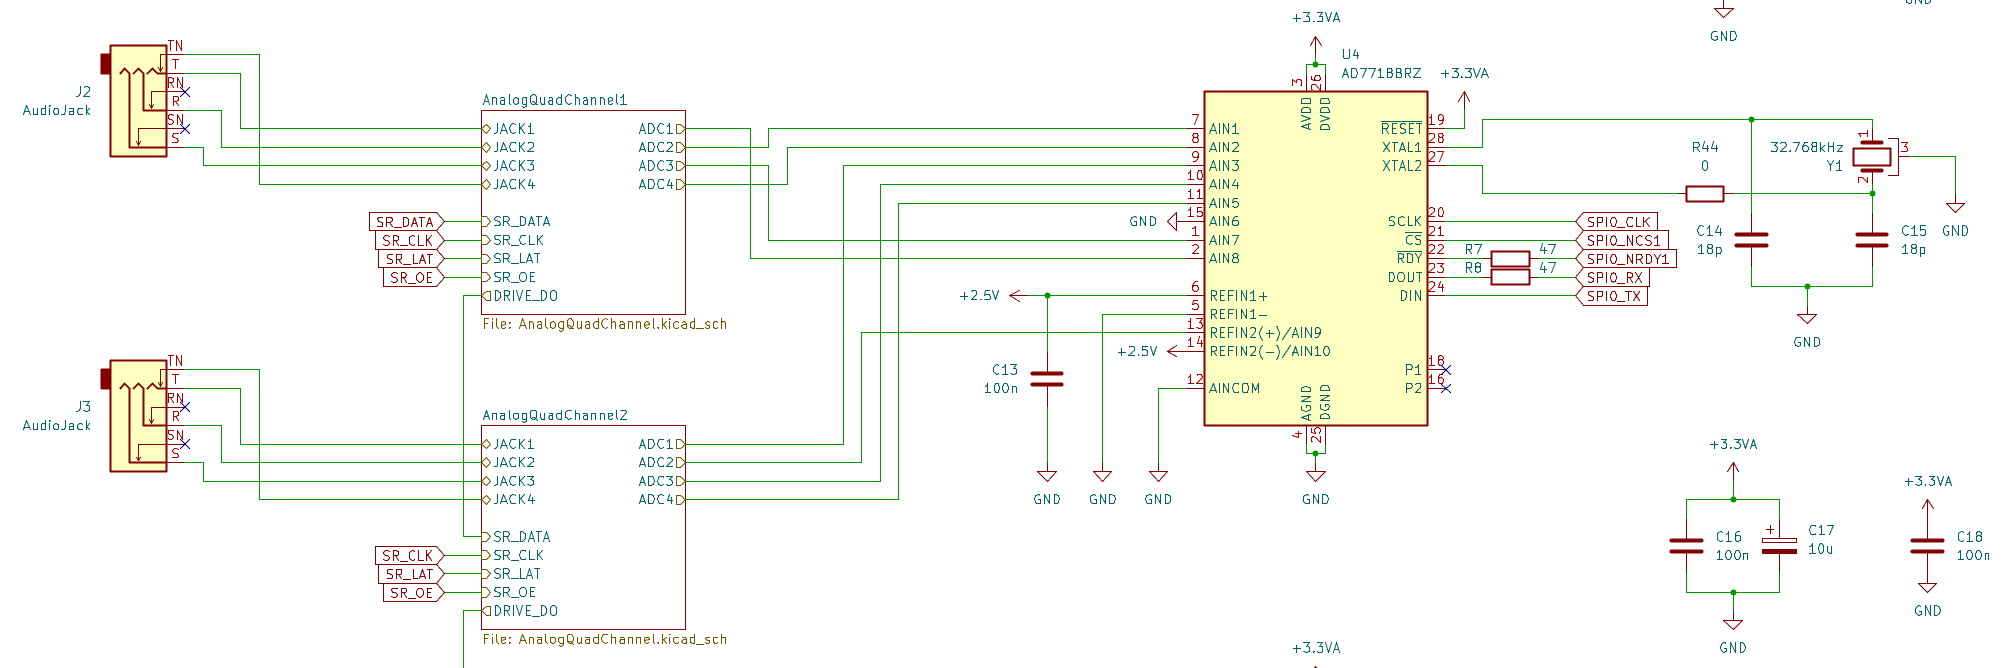
\includegraphics[width=\linewidth]{04-implementation/figures/adc}
  \titledcaption{ADCs}{\scaffoldinline{Name U4 and U5, the crystals, the reference connection to the \qty{2.5}{\volt} rail, the self-test inputs AIN6 and AIN10, and the SPI and ready signals to the microcontroller. Source: KiCad sheet \code{hardware/AnalogFrontend.kicad\_sch}; enlarge or split if the labels are not readable at text width.}}
  \label{fig:adc}
\end{figure}

\scaffold{
  \textbf{Paragraph 2, the filter and its settling.} The AD7718 is a sigma-delta ADC with a sinc\textsuperscript{3} decimation filter \cite{adi2001ad7718}. With chopping disabled, which the firmware uses for channel throughput, the output rate is programmable from \qty{16.06}{\hertz} to \qty{1365.33}{\hertz}; a channel change counts as a synchronized step and needs three conversion periods to settle \cite{adi2001ad7718}. Explain the consequence that shapes the whole firmware: every reading that changes the channel costs three conversion periods, independent of how fast the analog input settles. Mention that the datasheet requires recalibration after gain or temperature changes in this mode, and that the firmware calibrates once at start-up and measures its own rails (\cref{sec:pair-measurement}).
}

\scaffold{
  \textbf{Paragraph 3, the SPI interface.} Every SPI and shift-register line has a \qty{47}{\ohm} series resistor at its driver to slow the edges and damp reflections on the two-layer board. A chip-select guard of \qty{10}{\micro\second} before and after every transfer was found sufficient on the PCB, where the breadboard needed \qty{50}{\micro\second} and showed outlying codes otherwise; the firmware skips the control-register write when the channel does not change. Two driver bugs found on the breadboard are worth one sentence each: the ready line was polled before the chip had registered the conversion command, which corrupted the calibration, and toggling chip select too quickly made the chip lose synchronization.
}

\openquestion{Choice of 47 Ohm}{
  A design session recommended \qtyrange{22}{33}{\ohm}; the board has \qty{47}{\ohm}. Give the reason for the value.
}
